\section{面向对象建模}

\subsection{面向对象分析}

\subsubsection{现实世界的复杂模型}
\begin{itemize}
    \item 复杂总是简单部分的组合
    \item 简单部分又是更简单部分的组合
    \begin{itemize}
        \item 简单组成复杂的过程存在层次性
    \end{itemize}
    \item 每个最小简单部分独立负责完成一系列相关任务
    \item 相比较而言,每个组合内部各部分的关系比其内部与外部的关系都更紧密
    \item 各个部分通过一致的接口进行组合,即一个部分对其它部分的所知仅仅是接口
\end{itemize}

\subsubsection{映射现实模型的面向对象思想}
\begin{itemize}
    \item 任何系统都是能够完成一系列相关目标和任务的对象
    \begin{itemize}
        \item 对象完成一个任务时会请求一系列其他对象帮助其完成一些子目标
        \item 其他对象为了完成其任务又会请求将子目标更细分为子子目标,并请求其他对象帮助完成
        \item 子目标的分解和责任分担一直进行直到最后产生的子部分可以映射到计算实体
    \end{itemize}
\end{itemize}

\vspace{-0.8em}
\begin{multicols}{3}
    \begin{itemize}
        \item 计算实体:对象
        \item 层次关系:继承/关联、聚合/组合
        \item 组合接口:一个对象暴露的接口
    \end{itemize}
\end{multicols}
\vspace{-1em}

\subsubsection{基于UML的面向对象分析}
UML是以Booch方法、OOSE方法和ONT方法为基础,发挥3种方法的互补性,互相取长补短,并吸收了对象约束语言(Object Constraint Language, OCL)等其他技术之后产生的。
\begin{figure}[H]
	\centering
    \vspace{-0.5em}
	\includegraphics[width=0.7\textwidth]{img/Booch方法、OOSE方法、OMT方法与UML.png}
    \caption*{Booch方法、OOSE方法、OMT方法与UML}
    \vspace{-1em}
\end{figure}

在需求分析中涉及的UML技术有:
\vspace{-0.8em}
\begin{multicols}{2}
    \begin{itemize}
        \item 用例图(用例模型)
        \item 类图(对象模型)
        \item 交互图(顺序图/通信图,行为模型-对象协作)
        \item 状态图(行为模型-状态机)
        \item 活动图(行为模型-业务过程)
        \item 对象约束语言OCL
    \end{itemize}
\end{multicols}
\vspace{-1em}

面向对象分析与设计的关键是实现从用例模型到完全对象模型的过渡,包括下列几个步骤:
\begin{figure}[H]
	\centering
    \vspace{-0.5em}
	\includegraphics[width=0.9\textwidth]{img/面向对象方法的技术路线.png}
    \caption*{面向对象方法的技术路线}
    \vspace{-1em}
\end{figure}

\subsection{对象模型}

\subsubsection{对象}
对象是指在一个应用当中具有明确角色的独立可确认的实体 

每个对象都要包含
\begin{itemize}
    \item 标识:唯一的标识自己,对象模型使用对象的引用作为对象的标识
    \item 状态:对象的特征描述,包括对象的属性和属性的取值 
    \item 行为:对象在其状态发生改变或者接收到外界消息时所采取的行动 
\end{itemize}

常见的事物都可以是对象
\begin{itemize}
    \item 和系统存在交互的外部实体,例如人、设备、其他的软件系统等
    \item 问题域中存在的事物,例如报表、信息展示、信号等
    \item 在系统的上下文环境中发生的事件,例如一次外部控制行为、一次资源变化等
    \item 人们在与系统的交互之中所扮演的角色,例如系统管理人员、用户管理人员、普通用户等
    \item 和应用相关的组织单位,例如分公司、部门、团队、小组等
    \item 问题域中问题发生的地点,例如车间、办公室等
    \item 事物组合的结构关系,例如部分与整体的关系等
\end{itemize}

但是也有事物不是对象
\vspace{-0.8em}
\begin{multicols}{3}
    \begin{itemize}
        \item 无法界定的事物
        \item 纯粹的值
        \item 纯粹的行为
    \end{itemize}
\end{multicols}
\vspace{-1.2em}

\subsubsection{对象之间的关系}
系统中的对象不是孤立存在的,它们需要互相协作完成任务。对象之间这种互相协作的关系称为链接,它描述了对象之间的物理或业务联系。

链接通常是单向的,当然也有双向的链接存在。如果一个对象a存在指向b的链接,那就意味着a拥有对b的假设,关于b的行为和行为效果的假设。也就是说,b需要满足a的某些行为期望。

\subsubsection{类}
类是共享相同属性和行为的对象的集合,它为属于该类的所有对象提供统一的抽象描述和生成模板
\begin{itemize}
    \item 抽象描述称为接口,定义了类所含对象对外的(其他类和对象)的统一协议
    \item 生成模板称为实现,说明了类所含对象的生成机制和行为模式
\end{itemize}

类产生的关键是进行正确的分类,目前常见的类产生方法有数据驱动和职责驱动两种
\begin{itemize}
    \item 数据驱动:将具有相同属性的对象归为一类
    \begin{itemize}
        \item 产生自哲学上传统的经典分类理论:所有具有一个给定特性或共同特性集的实体组成一个类
    \end{itemize}
    \item 职责驱动:会依据事物的相似性而不是完全的相同性来进行事物的分类
    \begin{itemize}
        \item 产生自哲学上的概念聚类:使用概念描述而不是指定的特征来描述类别和事物,在进行事物分类时它会考虑概念之间的相似性,并将事物归入和其概念最为相似的类别
    \end{itemize}
\end{itemize}

\subsubsection{类之间的关系}
类与类之间的关系有继承、实现、依赖、关联、聚合和组合六种。
\vspace{-0.2em}

\begin{figure}[H]
	\setcounter{subfigure}{0}
	\centering
	\vspace{-1em}	
	\subfloat[关联的描述]{
		\begin{minipage}[t]{0.3\linewidth}
		\centering
		\includegraphics[width=\linewidth]{img/关联的描述.png}
		\end{minipage}
	}
    \hfill
	\subfloat[关联的其他特性描述]{
		\begin{minipage}[t]{0.67\linewidth}
		\centering
		\includegraphics[width=\linewidth]{img/关联的其他特性描述.png}
		\end{minipage}
	}

    \subfloat[聚合与组合示例]{
		\begin{minipage}[t]{0.48\linewidth}
		\centering
		\includegraphics[width=0.65\linewidth]{img/聚合与组合示例.png}
		\end{minipage}
	}
	\subfloat[继承关系图示]{
		\begin{minipage}[t]{0.49\linewidth}
		\centering
		\includegraphics[width=0.6\linewidth]{img/继承关系图示.png}
		\end{minipage}
	}
	\centering
	\vspace{-1em}
\end{figure}

\subsubsection{领域模型}
“领城”一词是指软件系统所处的同题域和业务范围。也就是说,在进行系统分析时,开发人员关注的仅仅是实际的业务范围,分析阶段产生的对象模型是关注用户问题域的对象模型,它被称为领域模型,又被称为领域类图、概念类图或分析类图。

领城模型中的类大多是概念类,是一个能够代表现实世界事物的概念,来自于对问题域的观察
\begin{itemize}
    \item 概念类之间存在指明语义联系的关联,这些关联通常不标记方向,也不标记关联端的可见性
    \item 概念类会显式的描述自己的一些重要属性,但不是全部的详细属性,而且概念类的属性通常没有类型的约束
    \item 概念类不显式的标记类的行为,即概念类不包含明确的方法
\end{itemize}

\begin{figure}[H]
	\centering
	\includegraphics[width=0.65\textwidth]{img/领域模型示例.png}
    \caption*{\textbf{领域模型(概念类图)示例}}
    \vspace{-1em}
\end{figure}

\subsection{建立领域模型}
领域模型的建立过程包括:识别候选对象与类、确定概念类、建立类之间的关联和添加类的重要属性。

\subsubsection{识别候选对象与类}
概念类分类列表:这种方法事先给出一个概念类的分类列表,从中发现对象
\begin{table}[H]
    \centering
    \begin{tabular}{|c|l|l|l|}
    \hline
    方式来源 & \multicolumn{1}{c|}{Shlaer-Mellor{[}Shlaer 1988{]}}            & \multicolumn{1}{c|}{Ross{[}Ross 1987{]}}                                     & \multicolumn{1}{c|}{Coad-Yourdon{[}Coad 1990{]}}                                   \\ \hline
    分类列表 & \begin{tabular}[c]{@{}l@{}}有形的事物\\ 角色\\ 事件\\ 交互功能\end{tabular} & \begin{tabular}[c]{@{}l@{}}人\\ 地点\\ 事物\\ 组织:集合体\\ 概念\\ 事件:需要被记录\end{tabular} & \begin{tabular}[c]{@{}l@{}}结构\\ 其他系统\\ 设备\\ 事件:需要被记录\\ 角色\\ 地点\\ 组织单位\end{tabular} \\ \hline
    \end{tabular}
    \caption*{常见的概念类分类}
    \vspace{-1em}
\end{table}

利用概念类分类列表发现对象和类的示例
\begin{figure}[H]
	\centering
    \vspace{-0.5em}
	\includegraphics[width=0.75\textwidth]{img/利用概念类分类列表发现对象和类的示例.png}
    \vspace{-1em}
\end{figure}


名词分析:从文本描述中识别出有关的名词和名词短语,然后从中发现对象
\begin{figure}[H]
	\centering
    \vspace{-0.5em}
	\includegraphics[width=0.9\textwidth]{img/利用名词分析发现候选对象和类.pdf}
    \vspace{-1em}
\end{figure}

\subsubsection{确定概念类}
确定概念类的准则
\begin{itemize}
    \item 如果候选对象既维持一定的状态,又依据状态表现一定的行为,那么它就应该是一个独立存在的对象
    \item 如果候选对象只有状态没有行为,那么就要分析它的状态是否是系统需要的数据
    \begin{itemize}
        \item 如果系统需要它的状态数据,那么该候选对象就应该作为其他对象的属性出现在最终的领域模型当中
        \item 否则,该候选对象应该被摈弃
    \end{itemize}
    \item 如果候选对象只有行为没有状态,那么往往意味着需求信息的遗漏
    \item 既没有状态也没有行为的候选类很少会出现,即使出现也可以很容易地做出将其摈弃的决定
\end{itemize}

\subsubsection{建立类之间的关联}
建立类之间的关联时,要注意下列原则
\begin{itemize}
    \item 保证类之间协作所必需的可见性
    \item 适当使用问题域内的关联,增强领域模型的可理解性
    \item 不要在关联的识别上花费太多的时间,识别概念类比识别关联更加重要
    \item 避免显示冗余和导出的关联
\end{itemize}


\subsubsection{添加类的重要属性}
这些属性往往是实现类协作时必要的信息,是协作的条件、输入、结果或过程记录。

在添加概念类的属性时通常遵循用户的描述方式,不进行类型和约束的严格定义。

\begin{figure}[H]
	\centering
    \vspace{-0.5em}
	\includegraphics[width=0.55\textwidth]{img/添加了属性的领域模型示例.png}
    \caption*{添加了属性的领域模型示例}
    \vspace{-1em}
\end{figure}


\subsubsection{领域模型的分析作用}
\begin{itemize}
    \item 发现数据方面的需求缺陷与不足,表现为数据的定义、加工与使用
    \item 用例之间是互补的,有些用例的数据缺陷可以在其他用例的领域模型中得到补充
\end{itemize}

\begin{figure}[H]
	\centering
	\includegraphics[width=0.95\textwidth]{img/领域模型的分析作用.pdf}
    \vspace{-1em}
\end{figure}


\subsection{行为模型——交互图}
\begin{itemize}
    \item 交互图是以一组对象为中心的交互描述技术
    \item 描述在特定上下文环境中一组对象的交互行为
    \item 通常描述的是单个用例的典型场景
    \item 交互图中的每一个交互都描述了环境中的对象为了实现某个目标而执行的一系列消息交换
    \item 顺序图和通信图是最常用的交互图
    \item 交互图中出现的对象应该在领域模型中有相应的对象存在
\end{itemize}

\subsubsection{顺序图}

\textbf{顺序图}可以突出消息的时间顺序,一个简单的顺序图如下所示
\begin{figure}[H]
	\setcounter{subfigure}{0}
	\centering
	\vspace{-0.5em}	
	\subfloat[一个简单的顺序图图示]{
		\begin{minipage}[c]{0.67\linewidth}
		\centering
		\includegraphics[width=\linewidth]{img/一个简单的顺序图图示.png}
		\end{minipage}
	}
    \hfill
	\subfloat[顺序图中不同消息类型的图示]{
		\begin{minipage}[c]{0.25\linewidth}
		\centering
		\includegraphics[width=\linewidth]{img/顺序图中不同消息类型的图示.png}
		\end{minipage}
	}
	\centering
	\vspace{-1em}
\end{figure}

顺序图还使用了一些表达复杂情景的组合片段
\begin{figure}[H]
	\centering
    \vspace{-0.2em}
	\includegraphics[width=0.65\textwidth]{img/组合片段示意图.png}
    \caption*{组合片段示意图}
    \vspace{-1em}
\end{figure}

顺序图的组合片段有以下几种
\begin{itemize}
    \item 选择(alternatives):操作符alt。表示要从多个行为中根据监护条件选择一个交互行为执行。在用例中存在分支流程时,往往要使用多选一组合片段。
    \item 可选(option):操作符opt。如果符合监护条件,那么片段内的交互行为就会得到执行,否则就不执行。
    \item 循环(loop):操作符loop。只要监护条件为真,片段内的交互行为就会被反复执行。
    \item 中断(break):操作符break。如果监护条件为真,片段内的交互行为就会被执行,并在执行后退出中断片段所在的顺序图,即如果中断发生,那么顺序图中中断片段之后的交互行为就不会得到执行。
    \item 并行(parallel):操作符par。并行片段内的不同交互行为可以不遵循顺序图的时间线顺序,可以并行、交织进行。
    \item 关键区域(critical region):操作符critical。区域内的交互行为是一个原子操作,一旦开始执行就必领执行完成, 在执行过程中不能被打断,例如其另一个并发片段中发生了Break行为,关键区域内容的交互行为仍然要执行完成后才能退出其所在的顺序图。
    \item 强顺序(strict sequencing):操作符strict。强顺序内的交互行为必须顺序执行。
    \item 弱顺序(weak sequencing):操作符seq。在弱顺序下:每个操作组内的交互行为要维持顺序关系;不同生命线上的不同操作组可以按照任何顺序执行;同一个生命线上的不同操作组要按照顺序执行。
\end{itemize}

\begin{figure}[H]
	\centering
    \vspace{-0.2em}
	\includegraphics[width=0.95\textwidth]{img/顺序图组合片段示例.png}
    \caption*{顺序图组合片段示例}
    \vspace{-1em}
\end{figure}


\subsubsection{系统顺序图}
\textbf{系统顺序图}将整个系统看作一个黑箱的对象,强调外部参与者和系统的交互行为,重点展示系统级事件 
\begin{figure}[H]
	\centering
    \vspace{-0.2em}
	\includegraphics[width=0.7\textwidth]{img/系统顺序图示例.png}
    \vspace{-1em}
\end{figure}


\subsection{建立交互图}

\subsubsection{建立典型场景的系统顺序图}
为典型场景建立系统顺序图的一般步骤如下:
\begin{enumerate}[label=\arabic*.]
    \item 确定系统顺序图的上下文环境
    \item 找出参与交互的对象
    \item 根据发现的对象建立交互图框架。将对象平行排列,并添加对象的生命线
    \item 添加消息,描述交互行为:以消息的方式,将对象之间的交互行为描述出来,并建立行为间的顺序
\end{enumerate}

\begin{figure}[H]
	\centering
    \vspace{-0.2em}
	\includegraphics[width=0.8\textwidth]{img/系统顺序图的建立示例.png}
    \caption*{系统顺序图的建立示例}
    \vspace{-1em}
\end{figure}


\subsubsection{建立用例(多场景)的系统顺序图}
先为主流程场景建立基础的系统顺序图,然后根据分支场景与异常场景的分支点、异常点,建立组合片段描述
\begin{figure}[H]
	\centering
    \vspace{-0.2em}
	\includegraphics[width=0.65\textwidth]{img/多场景的系统顺序图示例.pdf}
    \caption*{多场景的系统顺序图示例}
    \vspace{-1em}
\end{figure}


\subsubsection{建立详细顺序图}
对简单项目进行需求分析时,建立系统顺序图描述就足够了。如果项目比较复杂,系统顺序图中的交互行为粒度太大,可以考虑适度使用详细顺序图。

建立详细顾序图的关键是正确识别参与交互的对象,这个可以借鉴领域模型的工作。一个用例的详细顺序图中参与对象应该与该用例的领域对象是一致的。

详细顺序图仍然只是分析模型,因为它没有添加设计因素,所以到了设计阶段还需要被设计师继续细化,添加界面、数据模型等设计要素。

\begin{figure}[H]
	\centering
    \vspace{-0.2em}
	\includegraphics[width=0.95\textwidth]{img/详细顺序图示例.png}
    \caption*{详细顺序图示例}
    \vspace{-1em}
\end{figure}


\subsubsection{交互图的分析作用}
\textbf{建立交互图时最常发现的问题是系统的交互行为缺失。}

\textbf{组合片段和消息描述可能会发现行为数据的问题。}如果一个交互消息的数据内容在领域模型中没有描述,就意味着其数据内容是缺失的。如果组合片段监护条件使用的数据内容在领域模型中没有描述,也意味着其数据内容的缺失。


\subsection{行为模型——状态图}

\subsubsection{状态图概论}
状态图是以状态机理论为基础建立的对系统行为的描述手段
\begin{itemize}
    \item 状态机是以“状态”概念为基础解释系统行为的一种技术
    \item 有限状态机FSM(Finite State Machine)是用于建模的最简单的状态机
    \item 在FSM技术基础之上,发展出了多种分支技术(FSM, STD, Yourdon, SDL, STM, SC),UML的状态图SD (State Diagram)也是其中之一
\end{itemize}

状态图主要用于描述重要而且复杂的对象的所有行为,这个对象的行为通常要涉及很多(甚至大部分)的用例

\subsubsection{有限状态机}
状态机理论
\begin{itemize}
    \item 状态机理论认为,系统总是处于一定的状态之中。而且,在某一时刻,系统只能处于一种状态之中。
    \item 系统在任何一个状态中都是稳定的,如果没有外部事件触发,系统会一直持续维持该状态。
    \item 如果发生有效的触发事件,系统将会响应事件,从一种状态转移到唯一的另一种状态。
\end{itemize}

如果能够罗列出系统所有可能的状态,并发现所有有效的外部事件,那么就能够从状态转移的角度完整的表达系统的所有行为。

有限状态机可以被看作是一个5元组:$\mathrm{FSM}=(Q,\; \Sigma,\; \delta,\; q_0,\; F)$,其中:
\vspace{-0.8em}
\begin{multicols}{2}
    \begin{itemize}
        \item $Q$是系统所有可能的状态集合
        \item $\Sigma$是系统所有可能面对的触发事件
        \item $\delta$是状态转移两数。
        \item $q_0\in Q$是系统的初始状态
        \item $F\subset Q$是系统可能的结束状态的集合
    \end{itemize}
\end{multicols}
\vspace{-1em}

\subsubsection{状态图实例}
简单示例
\begin{figure}[H]
	\setcounter{subfigure}{0}
	\centering
	\vspace{-0.5em}	
	\subfloat{
		\begin{minipage}[c]{0.49\linewidth}
		\centering
		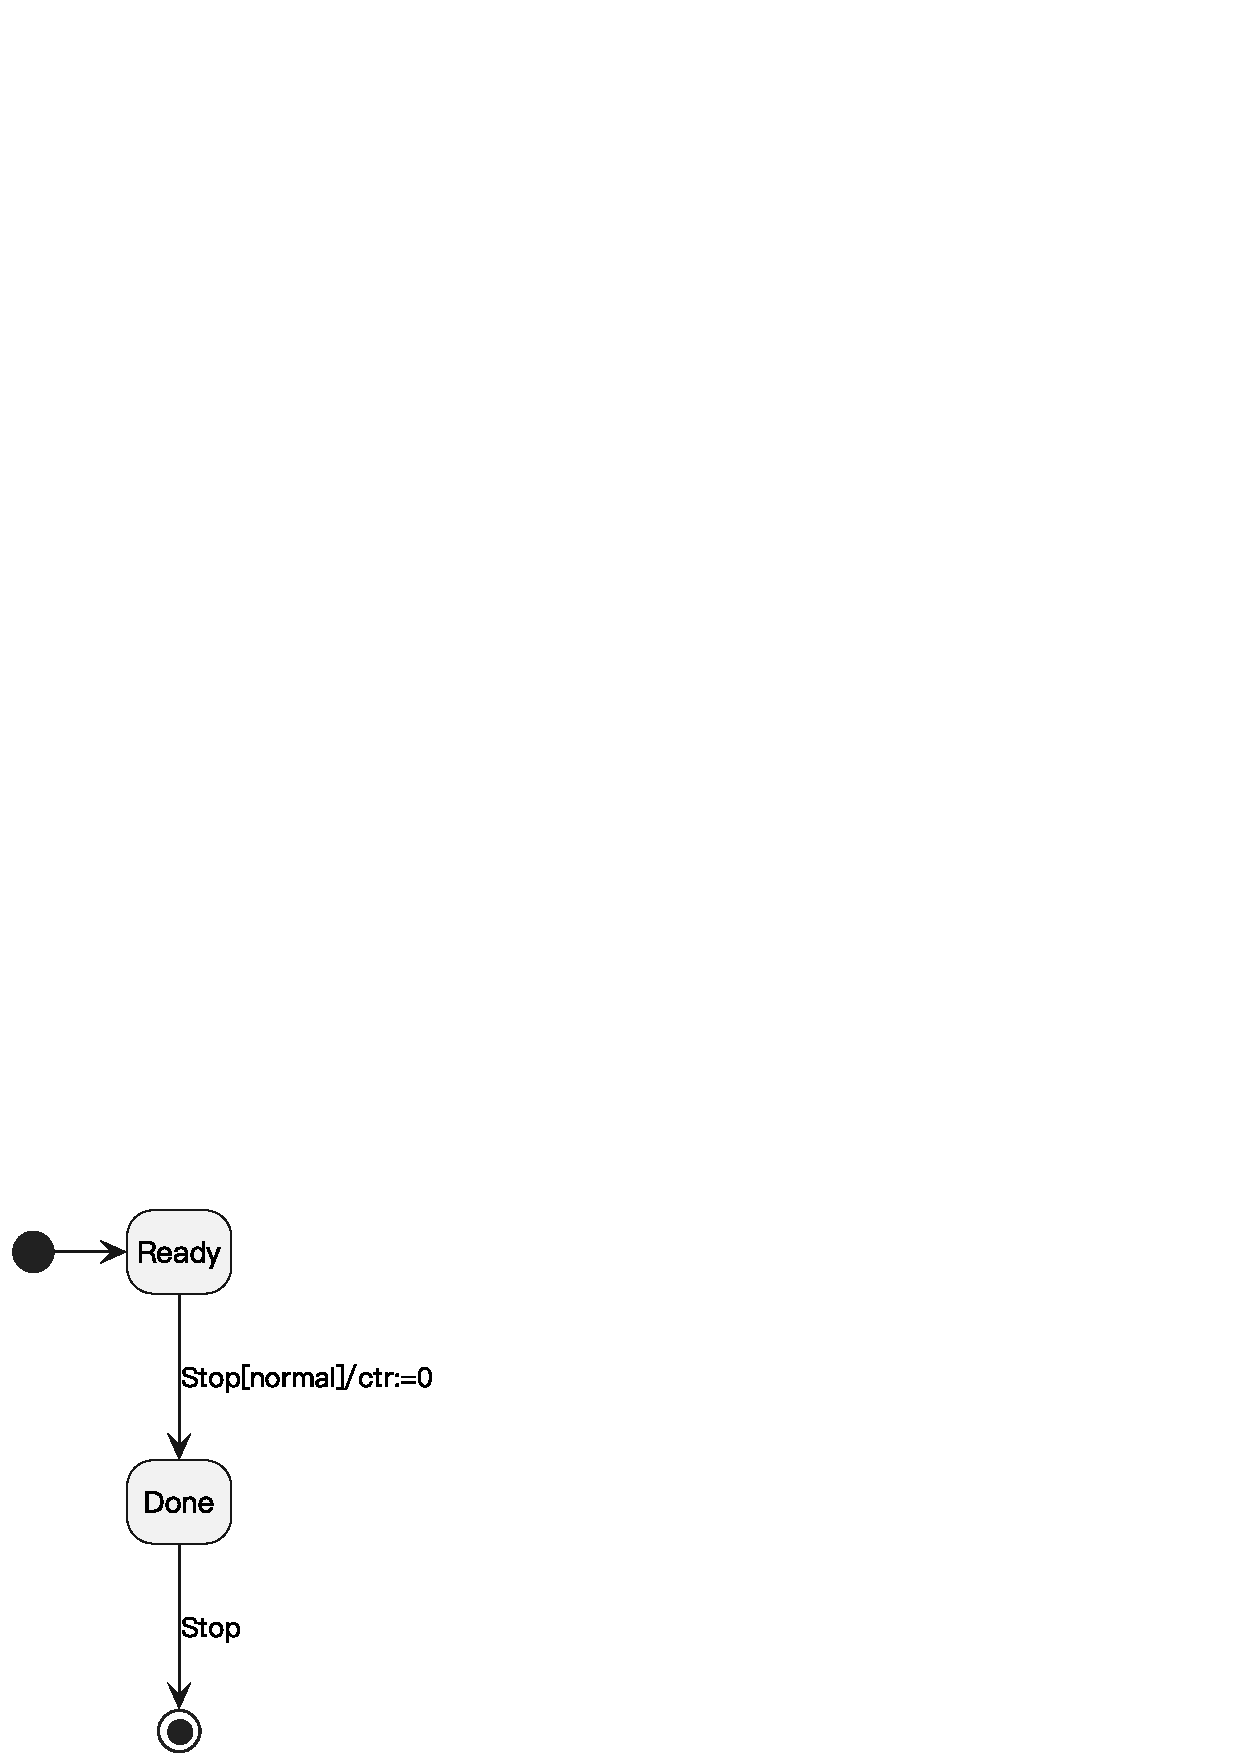
\includegraphics[width=\linewidth]{img/状态图简单示例1.pdf}
		\end{minipage}
	}
    \hfill
	\subfloat{
		\begin{minipage}[c]{0.48\linewidth}
		\centering
		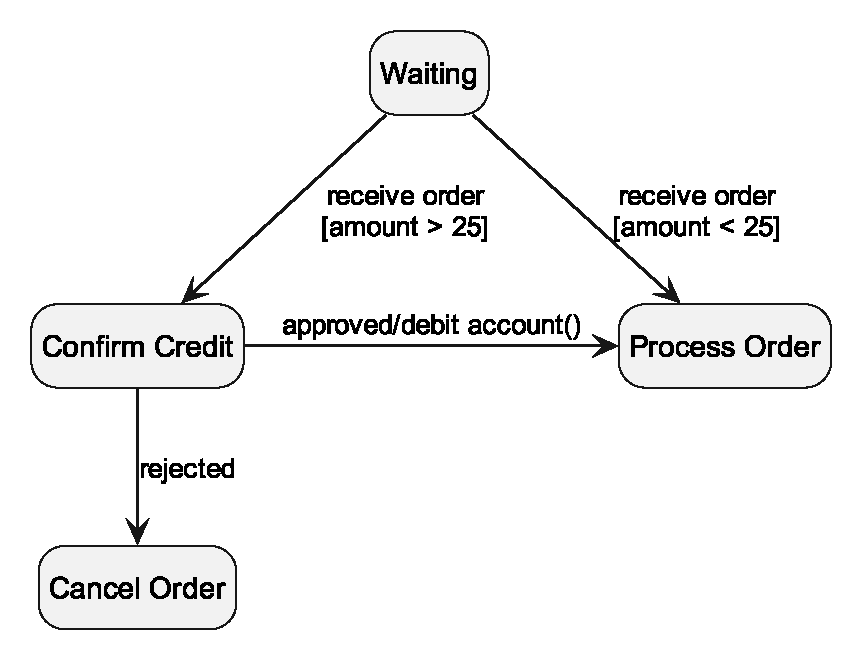
\includegraphics[width=\linewidth]{img/状态图简单示例2.eps}
		\end{minipage}
	}
	\centering
	\vspace{-1em}
\end{figure}

并发状态
\begin{figure}[H]
	\centering
    \vspace{-0.2em}
	\includegraphics[width=0.58\textwidth]{img/状态图并发状态.png}
    \vspace{-1em}
\end{figure}

入口与出口:子图的异常进入与退出
\begin{figure}[H]
	\setcounter{subfigure}{0}
	\centering
	\vspace{-0.5em}	
	\subfloat{
		\begin{minipage}[c]{0.25\linewidth}
		\centering
		\includegraphics[width=\linewidth]{img/状态图入口与出口1.png}
		\end{minipage}
	}
	\subfloat{
		\begin{minipage}[c]{0.4\linewidth}
		\centering
		\includegraphics[width=\linewidth]{img/状态图入口与出口2.png}
		\end{minipage}
	}
    \subfloat{
		\begin{minipage}[c]{0.32\linewidth}
		\centering
		\includegraphics[width=\linewidth]{img/状态图入口与出口3.png}
		\end{minipage}
	}
	\centering
	\vspace{-1em}
\end{figure}

决策选择与汇集点
\begin{figure}[H]
	\setcounter{subfigure}{0}
	\centering
	\vspace{-0.5em}	
	\subfloat{
		\begin{minipage}[c]{0.48\linewidth}
		\centering
		\includegraphics[width=\linewidth]{img/状态图决策选择.png}
		\end{minipage}
	}
	\subfloat{
		\begin{minipage}[c]{0.44\linewidth}
		\centering
		\includegraphics[width=\linewidth]{img/状态图汇集点.png}
		\end{minipage}
	}
	\centering
	\vspace{-1em}
\end{figure}

中止与历史状态
\begin{figure}[H]
	\setcounter{subfigure}{0}
	\centering
	\vspace{-0.5em}	
	\subfloat{
		\begin{minipage}[c]{0.4\linewidth}
		\centering
		\includegraphics[width=\linewidth]{img/状态图终止状态.png}
		\end{minipage}
	}
	\subfloat{
		\begin{minipage}[c]{0.55\linewidth}
		\centering
		\includegraphics[width=\linewidth]{img/状态图历史状态.png}
		\end{minipage}
	}
	\centering
	\vspace{-1em}
\end{figure}


\subsection{建立状态图}

\subsubsection{基于状态转移矩阵建立状态图}
建立状态图的步骤如下:
\begin{itemize}
    \item 确定上下文环境
    \begin{itemize}
        \item 搞清楚状态的主体常见的状态主体有:类、用例、多个用例和整个系统
    \end{itemize}
    \item 识别状态,标记初始状态和结束状态
    \begin{itemize}
        \item 可能会不存在确定的初始状态和结束状态 
    \end{itemize} 
    \item 建立状态转换  
    \item 补充详细信息,完善状态图 
\end{itemize}

例:针对上面商品销售的示例, 可以按照如下示例建立POS类的状态图
\begin{table}[H]
    \centering
    \begin{tabular}{|c|c|c|c|c|c|c|c|}
    \hline
           & 授权 & 空闲 & 销售开始 & 商品信息显示 & 错误提示 & 列表显示 & 销售结束 \\ \hline
    授权     & Y  & Y  &      &        &      &      &      \\ \hline
    空闲     & Y  &    & Y    & Y      &      &      & Y    \\ \hline
    销售开始   &    &    &      & Y      &      &      &      \\ \hline
    商品信息显示 &    &    &      &        & Y    & Y    &      \\ \hline
    错误提示   &    & Y  &      &        &      &      &      \\ \hline
    列表显示   &    & Y  &      &        &      &      &      \\ \hline
    销售结束   &    & Y  &      &        &      &      &      \\ \hline
    \end{tabular}
    \caption*{建立状态转换示例}
    \vspace{-1em}
\end{table}

\begin{figure}[H]
    \vspace{-0.2em}
	\includegraphics[width=0.75\textwidth]{img/状态图建立示例.png}
    \vspace{-1em}
\end{figure}


% 设定尺寸单位
\setlength{\TPHorizModule}{\textwidth}
\setlength{\TPVertModule}{\textwidth}
 
% 排版文本框
\begin{textblock}{0.33}(0.925,0.95)
{\kaishu \small
\begin{compactenum}[1.]
    \item 顾客携带商品到銷售终端POS前
    \item 收银员开始一个新的销售处理
    \item 收银员输入物品项标识
    \item 系统记录销售的物品项列表并且显示物品描述、价格和总价
\end{compactenum}
\vspace{-0.65em}
收银员重复步骤$3\sim 4$,直至输入所有物品项
\vspace{-0.6em}
\begin{compactenum}[1.]
    \setcounter{enumi}{4}
    \item 系统显示最后的总价
    \item 收银员告诉顾客总价,要求顾客支付账款
    \item 顾客付款,系统结账
    \item 系统记录整个销售处理,更新立品座在目录
    \item 系统打印收据
    \item 顾客离开
\end{compactenum}
}\end{textblock}

\subsubsection{状态图的分析作用}
\begin{itemize}
    \item 如果状态图中发现有无法进入的状态或者无法跳出的状态,就意味着相应行为的缺失
    \item 如果一个状态在发生触发时转移路线不确定,就意味着监护条件数据缺失或者行为需要细化
    \item 如果应该建立的状态转移在需求内容中没有体现,就需要修正需求内容
    \item 如果应该存在的状态在需求内容中没有体现,也需要修正需求内容
\end{itemize}

\subsection{对象约束语言OCL}
对象约束语言OCL并不是UML中单独的一个模型,而是被应用在其他的模型当中,丰富其他模型语义

对象约束语言是一种无副作用的规约语言
\vspace{-0.8em}
\begin{multicols}{2}
    \begin{itemize}
        \item 以表达式的方式定义对其他模型元素的约束
        \item 约束和限制其他模型元素的行为和状态变化
        \item 不会修改任何其他模型元素的表述
    \end{itemize}
\end{multicols}
\vspace{-1em}

对象约束语言不是一种编程语言
\begin{itemize}
    \item 对象约束语言的首要定位是建模语言,因此它在保证一定表达能力的前提下,注重于语言的简洁性和抽象性
    \item 它无法被用来描述程序的控制逻辑和工作流程,它的表达式定义也无法在程序中得到直接的执行
\end{itemize}

对象约束语言主要由类型、表达式和保留关键字3部分组成。

\subsubsection{对象约束语言示例}
\begin{figure}[H]
	\setcounter{subfigure}{0}
	\centering
	\vspace{-0.5em}	
	\subfloat[使用概念类图的表示方法]{
		\begin{minipage}[t]{0.48\linewidth}
		\centering
		\includegraphics[width=\linewidth]{img/对象约束语言示例1.pdf}
		\end{minipage}
	}
    \hfill
	\subfloat[使用对象约束语言表示]{
		\begin{minipage}[t]{0.48\linewidth}
		\centering
		\includegraphics[width=\linewidth]{img/对象约束语言示例2.pdf}
		\end{minipage}
	}
    \caption*{限定客运航班只能由客运飞机承运,货运航班只能由货运飞机承运}
	\centering
	\vspace{-1em}
\end{figure}

\begin{figure}[H]
    \centering
    \vspace{-0.2em}
	\includegraphics[width=0.75\textwidth]{img/对象约束语言示例3.pdf}
    \caption*{限定航班到达机场}
    \vspace{-1em}
\end{figure}

\subsubsection{对象约束语言的应用}
对象约束语言在UML模型中有很多的用途,其中最常见的是用来定义UML模型元素的4类约束:不变量、前置条件、后置条件和监护条件。

\paragraph*{不变量}~{} \par
不变量是可以对UML类元施加的约束
\begin{itemize}
    \item 类元需要保持它的表达式取值在指定的时间范围内或者指定的条件下始终为“真”
    \item 最常见的是用来约束类的属性或者类的方法
\end{itemize}

\begin{figure}[H]
	\setcounter{subfigure}{0}
	\centering
	\vspace{-0.5em}	
	\subfloat[使用表达式描述]{
		\begin{minipage}[t]{0.3\linewidth}
		\centering
		\includegraphics[width=0.75\linewidth]{img/对象约束语言的应用不变量1.pdf}
		\end{minipage}
	}
    \hfill
	\subfloat[在UML图中直接添加带有<<invariant>>标签的特殊注释来进行说明]{
		\begin{minipage}[t]{0.65\linewidth}
		\centering
		\includegraphics[width=0.7\linewidth]{img/对象约束语言的应用不变量2.pdf}
		\end{minipage}
	}
    \caption*{限制Flight的时间小于4(小时)}
	\centering
	\vspace{-1em}
\end{figure}

\paragraph*{前置条件和后置条件}~{} \par
前置条件和后置条件是可以对类元的操作施加的约束
\begin{itemize}
    \item 前置条件要求类元在执行操作之前必须保证前置条件的表达式为真
    \item 后置条件要求类元在操作执行完成之后必须保证后置条件的表达式为真
\end{itemize}

\begin{figure}[H]
    \centering
    \vspace{-0.2em}
	\includegraphics[width=0.8\textwidth]{img/对象约束语言的应用前置条件和后置条件.pdf}
    \vspace{-1em}
\end{figure}

\paragraph*{监护条件}~{} \par
监护条件是对状态机模型中状态转移施加的约束
\begin{itemize}
    \item 在状态机到达转移点时,监护条件的表达式需要根据实际状态进行评估,并只有在表达式实际取值为“真”的情况下才进行转移
\end{itemize}

\begin{figure}[H]
    \centering
    \vspace{-0.2em}
	\includegraphics[width=0.8\textwidth]{img/对象约束语言的应用监护条件.pdf}
    \vspace{-1em}
\end{figure}


\subsection{使用对象约束语言建立契约说明}
不需要为所有的系统行为都定义操作契约,可以有选择的为其中的一部分系统行为定义操作契约
\vspace{-0.8em}
\begin{multicols}{2}
    \begin{itemize}
        \item 涉及到很多状态变化的复杂行为
        \item 因果关系比较微妙的模糊行为
    \end{itemize}
\end{multicols}
\vspace{-1em}

可以从下面几个角度进行约束的发现工作:
\begin{itemize}
    \item 不变量:系统行为中所涉及的敏感状态,这些状态的改变往往会产生广泛的连锁反应
    \begin{itemize}
        \item 不可改变的属性、不可改变的关联关系
    \end{itemize}
    \item 前置条件:行为发生和顺利完成所需要的系统的状态条件
    \begin{itemize}
        \item 合法的参数
        \item 有效的状态:对象的存在状态、对象的属性取值、有效的关联关系
    \end{itemize}
    \item 后置条件:行为顺利完成之后引起的系统状态改变
    \begin{itemize}
        \item 有效状态的改变:对象的存在状态、对象的属性取值
        \item 关联关系的改变
    \end{itemize}
\end{itemize}

\begin{figure}[H]
    \centering
    \vspace{-0.2em}
	\includegraphics[width=0.85\textwidth]{img/使用对象约束语言建立契约说明.pdf}
    \caption*{对左图中的系统行为“输入物品项”,可以进行操作契约的描述如右图所述}
    \vspace{-1em}
\end{figure}